\chapter{Managing User Steering Action Data in Workflow Scripts}
\label{chap_dfadapter}

The first instantiation of WfSteer, called DfAdapter,
aims at allowing for tracking steering actions with low execution overhead in large-scale workflow scripts.
DfAdapter is a lightweight
tool whose goal is to capture provenance of online steering actions in dataflows and storing the related dataflow provenance to enable understanding of the impacts of the actions.
Section \ref{dfadapter_utilization_methodology} presents DfAdapter's methodology and general conceptual architecture; Section \ref{wfscript_system-design-principles} has the main system design principles followed by DfAdapter; Section \ref{dfadapter-implementation-details} has implementation details; Section \ref{dfadapter_utilization} shows how DfAdapter is utilized; and Section \ref{overhead-analysis-section}
concludes with a methodology to analyze
the incurred overhead.
% Parts of the content of this chapter have been originally published in the Future Generation Computer Systems journal in 2019 \cite{souza_keeping_2019}.


\section{Methodology and General Architecture}

\subsubsection{Methodology}
\label{dfadapter_utilization_methodology}

In this section, we briefly describe a methodology that defines the  steps that need to be followed to enable steering action data management in an adaptable application.
Some of these steps occur offline, before the execution starts, whereas others occur online.
The offline steps are mainly related to manually inserting the APIs calls in the workflow to capture data when the workflow executes.
We extend our previous methodology \cite{Silva2018Capturing} to add steering action data management support. The methodology
presented in this thesis has been adapted from our paper \citet{souza_keeping_2019}.
Table~\ref{tab:methodology}
summarizes the high-level steps for enabling tracking of steering actions.

\begin{table}[H]
\caption{Methodology for workflow steering.}
\label{tab:methodology}
\begin{tabular}
{|
  M{.10\textwidth}|
  M{.60\textwidth}|
  M{.20\textwidth}|
}
\Xhline{4\arrayrulewidth}
1 & Identify the workflow                      & \multirow{3}{*}{Before execution} \\
%\Xhline{0.5\arrayrulewidth}
2 & Add analysis points in the workflow   &                                   \\
%\Xhline{0.5\arrayrulewidth}
3 & Add adaptation points in the workflow &                                   \\
\Xhline{3\arrayrulewidth}
4 & Online data analysis                       & \multirow{4}{*}{During execution} \\
%\Xhline{0.5\arrayrulewidth}
5 & Execute a steering action                  &                                   \\
%\Xhline{0.5\arrayrulewidth}
6 & Steering action data management            &                                   \\
%\Xhline{0.5\arrayrulewidth}
7 & Steering action data analysis              &                                   \\
\Xhline{4\arrayrulewidth}
\end{tabular}
\end{table}

In Step 1, users identify inputs and outputs of relevant parts of their application
that form a workflow. That is, they identify and specify the data transformations, the datasets, and the data derivation paths.
In Step 2, API calls are inserted in the workflow to add \textit{analysis points}, which are the regions in the workflow
that contain relevant (for the users) data for analysis at runtime.
These data consist of relevant input and output data elements in the dataflow, to be analyzed online, either for monitoring or interactive analysis.
In Step 3, users identify parts of the workflow that can be dynamically adapted at runtime and add \textit{adaptation points} in those parts.
    Adaptation points should be added to safe points of the workflow to avoid execution or data inconsistencies.
    Usually, users know where to add adaptation points.
    A typical example occurs in iterative workflows where each new iteration is an opportunity to redefine parameters or input datasets preset beforehand. In this case, an adaptation point is added at the beginning of the iteration. Each iteration is often executed as a whole. When a user adapts, the adaptation will take effect only at the next iteration, rather than changing values during an iteration. This helps to make data and execution consistent with what the user decided to adapt during the iteration.
    After these three initial offline steps, the workflow is submitted to parallel execution in an HPC machine.
In Step 4, the workflow data specified in the analysis points at Step 2 are captured and can be analyzed online.
In Step 5, based on the analyses, users may decide to execute a steering action.
In Step 6, the system captures the steering action data and relates the steering action to the rest of the workflow data being captured, and stores in the database.
Finally, in Step 7, users analyze the consequences of their actions relating to domain-specific relevant data and execution data.
In our experiments (Sec. \ref{sec_exps_wfscripts}), we provide concrete examples of how these steps are carried out in a real workflow.

\subsubsection{General Conceptual Architecture}

In this section, we present DfAdapter's general conceptual architecture (Figure \ref{fig:general_arch}). We describe its components as follows.

\begin{figure}[H]
    \centering
    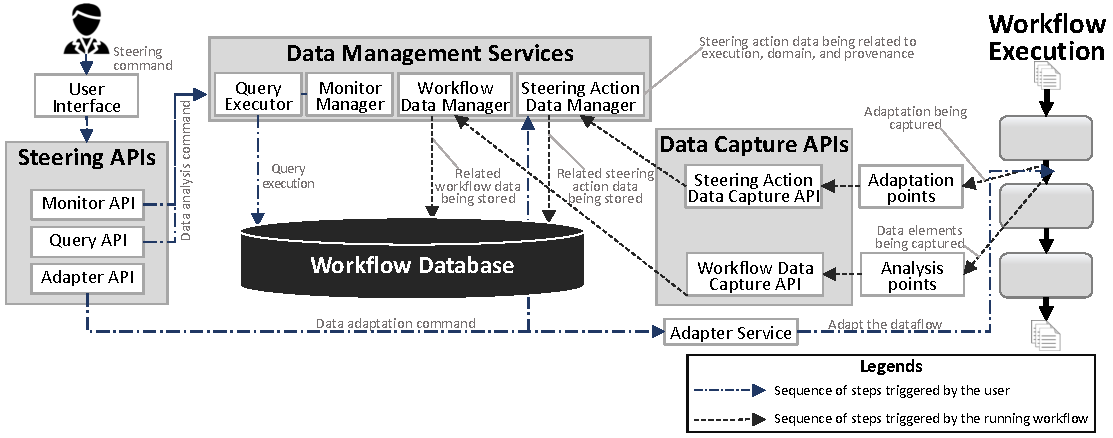
\includegraphics[width=\textwidth,keepaspectratio]{img/chap5_gen_arch.pdf}
    \caption{DfAdapter's General Conceptual Architecture.}
    \label{fig:general_arch}
\end{figure}


\subsubsubsection{Data Capture APIs}

The Data Capture APIs are \textit{Workflow Data Capture API} and \textit{Steering Action Data Capture API}.
The Workflow Data Capture API has the programming interfaces containing the methods to insert workflow data (mainly domain data values) into the workflow database. Calls to this API are inserted in the analysis points in the workflow.
Steering Action Data Capture API has the programming interfaces with the methods to capture steering action data, when a steering action is issued by the user. Calls to this API are inserted in the adaptation points.
These APIs are inserted in the workflow, called by workflow at runtime, and call the steering data management services.

\subsubsubsection{Data Management Services}

There are three main services composing the Steering Data Management Services: \textit{Query Executor}, \textit{Monitor Manager}, \textit{Workflow Data Manager}, and \textit{Steering Action Data Manager}.
The Workflow Data Manager is responsible for receiving the calls from the Workflow Data Capture API with the captured data during workflow execution.
Then, it provides the data relationships to the other data in the workflow database, integrating provenance, domain, and execution data, and finally stores the related workflow data in the workflow database.
The Steering Action Data Manager listens to calls from the Steering Action Data Capture API.
This service is responsible for
consistently adding the data relationships between the captured steering action and the remainder of the workflow data, and storing the related steering action in the workflow database.

The Query Executor is only called by the Steering API. When the client, \ie{} the user or a data visualization application, performs a data analysis command, like analysis or interactive analysis, the Query Executor is issued.
It then builds the needed queries according to the client's requests and executes the query to the DBMS managing the
workflow database to retrieve the requested data. The Monitor Manager is to implement the adaptive monitoring concepts (Sec. \ref{sec_adaptive_monitoring_concepts}). The user programs the monitoring query by using the interface that calls the Monitor API, which calls the Monitor Manager service. This service is responsible for managing the monitoring queries, for submitting the queries to the Query Executor at each time interval programmed by the user, and for returning the query results to the requesting client, \ie{} the Monitor API.

\subsubsubsection{Steering APIs}

The Steering APIs are composed of three APIs: \textit{Monitor API}, \textit{Query API}, and \textit{Adapter API}.
The Monitor and Query APIs call the Query Executor for data analysis, either for workflow analysis or for interactive analysis, respectively.
They contain programming interfaces that allow users to submit queries to the Query Executor.
The Adapter API has the interfaces for calling the Adapter Service, which is the component in the adaptable application that knows how to adapt the workflow (see the definition of the Adapter software service in Sec. \ref{sec:prov_dfa_general_concepts}).
The interfaces in the Adapter API are implemented according to the data communication implemented for the adaptable application, as we see in the next section (Sec. \ref{wfscript_system-design-principles}).
The Steering API's submodules are called by the user using the \textit{User Interface}, which concentrates the available commands the user can issue using the Steering API. It can be exposed as a command line interface, graphical user interfaces, or as a RESTful API.


\section{Design Principles}
\label{wfscript_system-design-principles}

In this section, we explain the core design principles followed
by DfAdapter.

\crossref{V1: nos wms, os requisitos são datflow; e no caso dos scripts, o que seria necessário?}
\textbf{Dataflow-oriented Data Capture and Analysis.} 
DfAdapter relies on a dataflow-oriented approach for workflows, as the one presented in 
Section \ref{subsec_datacentric}, as this is the fundamental basis for WfSteer to manage steering action data, as discussed in Chapter \ref{chap4}. DfAdapter needs that the domain data flowing in the dataflow are captured and stored in a workflow database, during execution, jointly with execution and provenance data (Sec. \ref{section_workflow_steering_db}).
Considering workflow scripts, DfAnalyzer \cite{Silva2017Raw,Camata2018In,silva_dfanalyzer:_2018} is a tool that can be coupled with scripts to capture runtime data, aware of the dataflow, and stores these captured data in a database ready for analysis during execution.
In the implementation section (Sec. \ref{dfadapter-implementation-details}), we explain how DfAdapter is combined with DfAnalyzer to provide rich runtime data analysis that integrates provenance, execution, domain, and steering action data.


\textbf{Asynchronous Service Calls.}
DfAdapter can be coupled to adaptable
applications, like the ones proposed by approaches that allow for online adaptation (Table \ref{tab:comparative_tables_systems})
or adaptable workflow scripts.
In either case, to enable steering action data analysis,
the Steering Action Data Capture API is used so it can be called from the adaptation points in the adaptable application.
Similarly, to enable online workflow data analysis,
Workflow Data Capture API calls are placed in analysis points in the workflow
script to capture data elements flowing in the dataflow and execution data of data
transformations.

Since CSE users typically discard any tool that can add significant overhead to their already long workflow executions, attaining low performance overhead is a basic requirement in DfAdapter.
For this, calls to DfAdapter are asynchronous,
meaning that when the user adapts the running workflow, the steering action data capture is done in such a way that the main computational
process will not wait until the steering action data are completely stored.
The same strategy is
followed for any added Workflow Data Capture API in the workflow. Also,
the most computationally costly components in DfAdapter, such as the
ones that relate and store steering action data in the database during workflow
execution, are deployed in separate hardware, different from where the
main computational process runs, but in the same internal network
(\eg{} the nodes in the HPC machine has local access to the node that
runs the Data Management Services) to reduce communication costs,
following \textit{in-situ} and \textit{in-transit} approaches
\cite{Bauer2016In}.
This avoids making DfAdapter and the main computational process compete
for resources.

% Adding adaptation points in an adaptable
% workflow means that in those points there will be data communication
% between the running workflow and DfAdapter, the Steering Action Data Manager service more specifically,
% so that when the user adapts, the steering action data will be captured, related, and stored.

\textbf{Data Communication between DfAdapter
and the Running Workflow.}
\label{data_comm_impl}
To be able to capture steering action data, DfAdapter needs to
access the data being adapted in a steering action.
For this, we characterize here the data communication between the Adapter Service and the adaptable application.
By analyzing the state-of-the-art (Chapter \ref{chap3}), we identified three ways to implement such data communication.
To access the data being adapted, DfAdapter needs to intercept this communication. We characterize these
implementations as follows.

\emph{i. File-based checks ---} This is a simple yet widely used way to
implement data communication \cite{Bauer2016In}.
In this case, there are files in a storage resource that are accessible
both by the Adapter API and by the Adapter Service.
That is, the Adapter API modifies a file that is accessible by the running workflow.
When the program pointer in the running workflow reaches an adaptation point,
the Adapter Service verifies if files
were modified based on the last-modification date metadata provided by the file system API, in case of modification, the application is adapted.
Then, the Steering Action Data Manager service is called to relate and store the adaptation.
Although
file-based checks are a simple approach, it is widely used especially by
users that implement their own \emph{ad-hoc} way to make their
simulation steerable.
However, it requires that the Adapter API and the Adapter Service share access to files in a storage resource, which
may not be always possible. This is the way libMesh-sedimentation (Sec. \ref{sub_libmesh}), used in our experiments (Sec. \ref{chap6}), implements the data communication.

\emph{ii. Message passing ---} In this case, the Adapter API sends a message to the Adapter Service in the
running workflow. When the adaptation point is achieved, the Adapter Service verifies if a message has arrived and effectuates the
adaptation accordingly, and DfAdapter is called to relate and store the
steering action data.
MPI, sockets, or RESTful HTTP messages can be used as
communication protocol to implement this.
Many systems that enable adaptation use message passing to implement the data communication
\cite{Pickles2005practical,Figueira2004CS_LITE:,Knezevic2011Interactive}.
This is an alternative to file-based checks, as it does not require
files to be shared in a storage resource by the adapter's front and back
ends.

\emph{iii. DBMS-driven ---}
It is similar to file-based checks in the sense that
there is a DBMS that is accessible both by the Adapter API and the Adapter Service in the running workflow.
It is similar to message passing in the sense that it does
not require files to be shared in a storage resource.
Rather, data that
can be modified at runtime are managed by the DBMS that can even run
in-memory, depending on the DBMS.
In this implementation, when the user uses the user interface to adapt, the Adapter API modifies the data in the DBMS.
When the program pointer achieves the adaptation point in the running
workflow, the Adapter Service checks if the data have been modified, effectuates
the adaptation accordingly, and DfAdapter is called to relate and store the steering action data.
We tested this implementation in a synthetic workflow example using the parallel framework
Apache Spark and Redis, a lightweight in-memory Key Value store, as the
DBMS between the workflow and DfAdapter. The source code is available on
GitHub \cite{DfAdapterGitHubDfAdapter} and in Appendix \ref{dfadaptercode}.

\textbf{DBMS and Data Model for the Workflow Database.} DfAdapter
needs a DBMS to manage the workflow database. Several data models can
be used for workflow databases, such as graph and relational data
models. The usage pattern in DfAdapter is that the running workflow only
produces insertions to the database, while the user typically
runs provenance queries for online data analyses to support
decision-making, \ie{} \myabbrev{OLAP}{Online Analytical Processing} queries.
This usage pattern, both by
the running workflow and by the user, is benefited from column-oriented
relational DBMSs, as shown in previous works
\cite{Silva2017Raw,Camata2018In}.
Moreover, since there may be many appends to this database during
execution, the DBMS must be able to handle parallel requests from
clients. One available option for this is the open source DBMS MonetDB\footnote{https://www.monetdb.org}, which is the one currently in use by DfAdapter.

\section{Implementation Details}
\label{dfadapter-implementation-details}

This section describes the implementation details of DfAdapter. The steering action currently implemented in DfAdapter is the user-steered parameter tuning, which is by far the most supported one by user steering approaches, as we surveyed in Chapter \ref{chap3}.
Here we describe the sequence of steps that are executed to manage steering action data, as illustrated in the sequence diagram in Figure \ref{fig:dfadapter_seq_diagram}.
First, during the workflow execution, (0) the data
specified in the analysis points are sent to the Workflow Data Manager Service via
Workflow Data Capture API calls.
Then, (1) Workflow Data Manager service relates and stores
the data in the Workflow Database.
While the workflow
runs, the user can call Query or Monitor APIs to follow the
intermediate data results and decide for an adaptation action.
If the user
decides for an adaptation action,
(2) the user sends a steering command
using DfAdapter's steering command line interface (implemented as a program called \codefont{WfSteerCtl}), which (3) calls the
Adapter API,
which (4) calls the Steering Action Data Manager service, 
\crossref{L6: Fig 5.2 – acertar a figura do diagrama de sequencias para incluir o ack e bloqueio
} 
waits for the service callback, then (5) registers the beginning of an adaptation intention.
The Adapter API also (6)
communicates with the Adapter Service, which (7)  effectuates the adaptation.
When (8) the running
workflow notices that an adaptation occurred (\eg{} it verifies
that a file or a data structure, depending on the data communication
implementation, has been changed because of a steering action), the (9)
Steering Action Data Capture API inserted in the adaptation point is
called to send the captured adaptation data to the Steering Action Data Manager service.
(10) The service receives the call, relates the steering action with the workflow data being processed, and stores in the Workflow Database. 
After that, the workflow
continues to run, and finally
(11) the user can run user steering action analysis.

\begin{figure}[H]
    \centering
    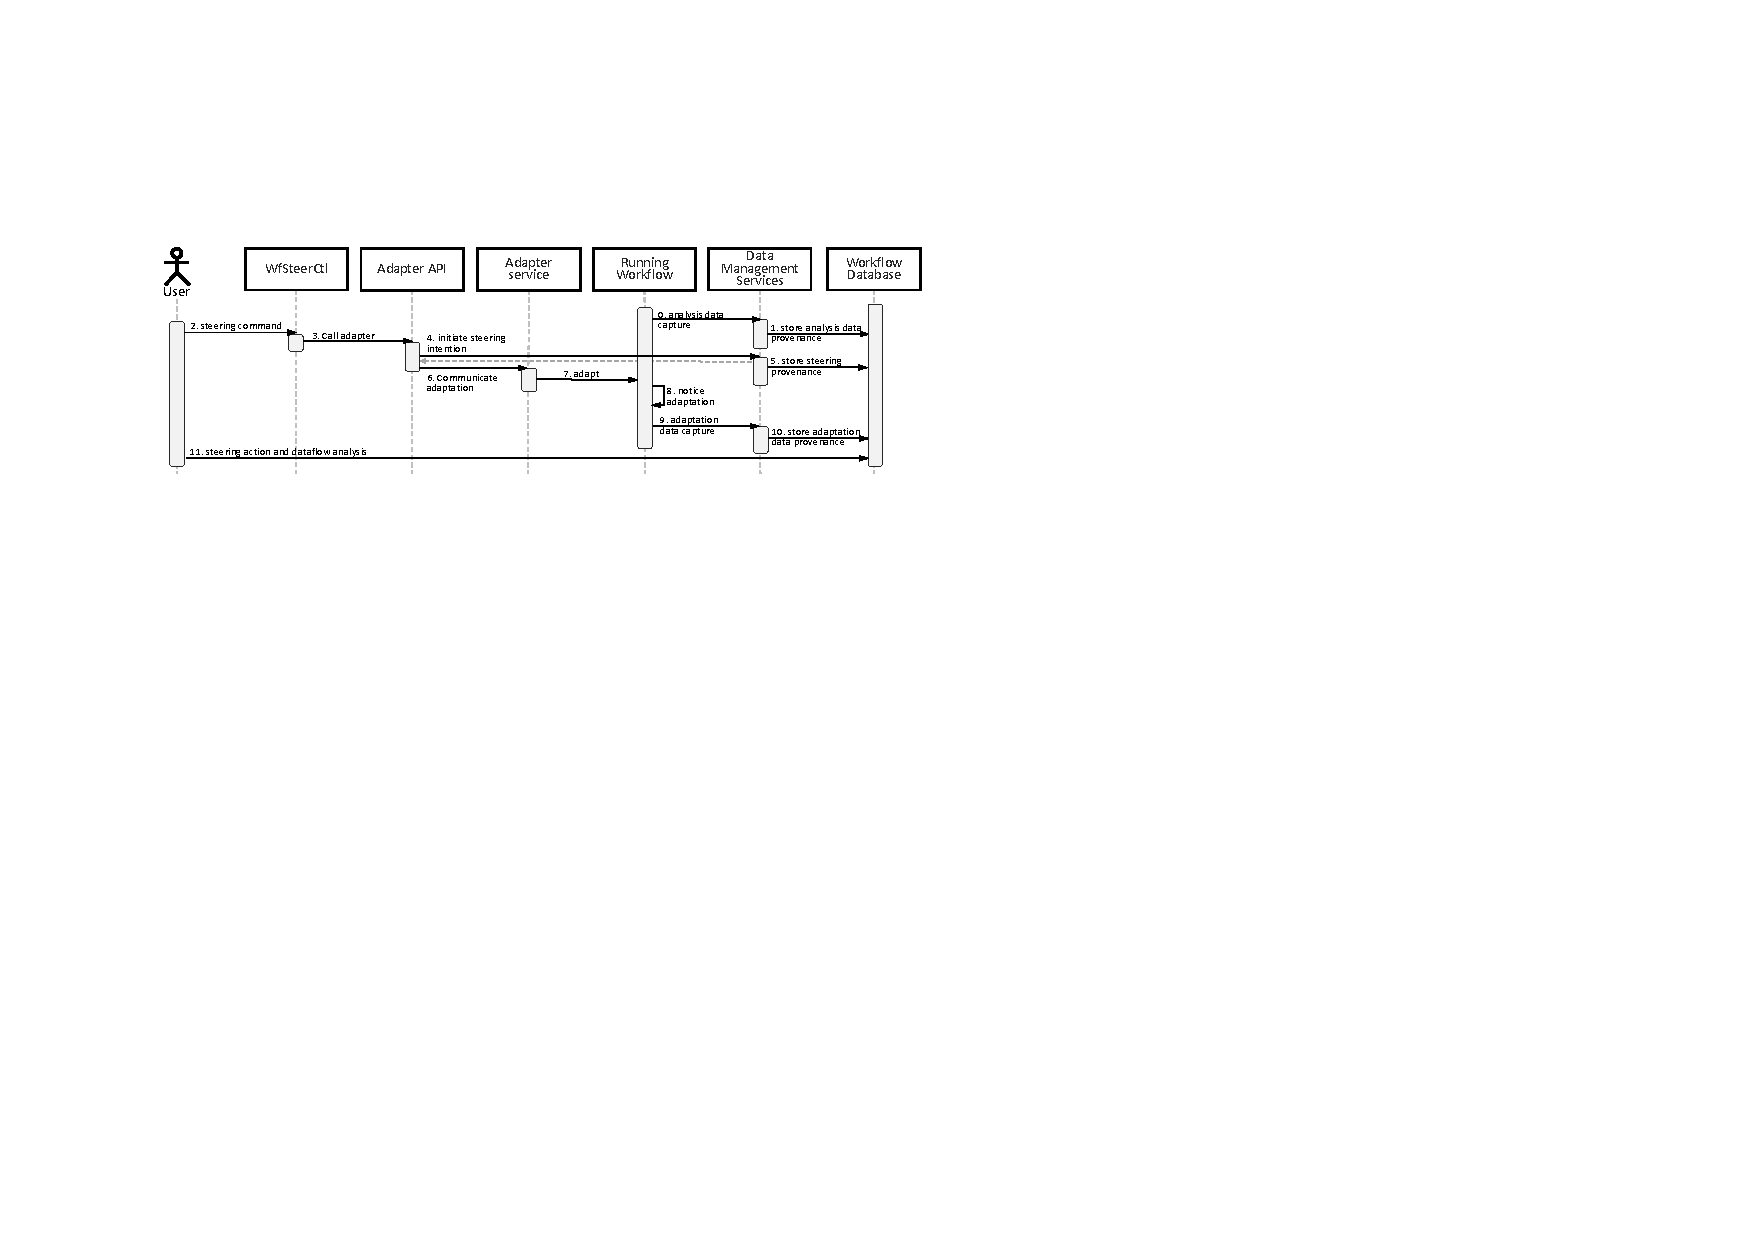
\includegraphics[width=\textwidth,keepaspectratio]{img/df_adapter_seq_diagram.pdf}
    \caption{Sequence diagram for managing steering action data with DfAdapter.}
    \label{fig:dfadapter_seq_diagram}
\end{figure}

The $Tune$ operator (Def. \ref{def:tune}) is implemented
to call the Steering Action Data Capture API. Before the call,
the steering action data need to be prepared.
Algorithm \ref{alg:alg_tune_operator} defines how the steering action data need to
be prepared before sending them to the Data Management Services.
The iteration data at the moment of the action is denoted by  $\xi$; the wall time at the moment of the
action is denoted by $t$; and the set of ordered pairs with
the old values for the tuned parameters are denoted by $\theta$.
The algorithm registers new domain data that
were modified in the adaptation as well as
 their corresponding old values. It captures current execution
data, iteration counter values (in case of iterative workflows), and
user data. Then, it stores user steering data relating to the rest of the workflow data
being continuously captured during workflow execution.


\begin{algorithm}
  \DontPrintSemicolon
  \begin{small}
  \KwIn{
  
  $I_{DS}$: The input dataset in the dataflow containing the parameters to be tuned.
  
  $\eta$: key-value data structure containing the parameters and their new values.
  
  $C <\text{optional}>:$ criteria to specify the data element that is being adapted.
  
  $\mu <\text{optional}>:$ metadata about the steering action, such as annotations.
  }


import data\_capture\_api\;

$\theta \leftarrow \varnothing$\;
$\xi  \leftarrow \varnothing$\;
$\Gamma \leftarrow $ data\_capture\_api.get\_running\_tasks()\;
$U \leftarrow $ data\_capture\_api.get\_user()\;
$t \leftarrow $ data\_capture\_api.get\_current\_wall\_time()\;
$current\_data\_element \leftarrow $ data\_capture\_api.get\_element$(I_{DS},C)$\;
$attribute\_semantics \leftarrow $ data\_capture\_api.get\_semantics$(I_{DS})$\;

\For{\textbf{all key-value pairs} $(p, current\_value)$ \textbf{ in } $current\_data\_element$}{
    
    \If{$p \in keys(\eta)$}{
        $\theta[p] \leftarrow current\_value$\;
        \If{$p \in attribute\_semantics[L_I] \textbf{ and } \xi=\varnothing$}{
            \tcp*{Tuning a loop attribute. Get iteration data}
            $\xi \leftarrow $ data\_capture\_api.get\_current\_iteration\_data$(I_{DS})$
            
        }
    }
    
}
data\_capture\_api.send\_steering\_action\_data$(
    I_{DS},
    \eta,
    C,
    U,
    \Gamma,
    \mu,
    \xi,
    t,
    \theta
)$


  \end{small}
 \caption{Capturing User Steering Action Data for $Tune$.}
 \label{alg:alg_tune_operator}
\end{algorithm}

\subsubsection{Workflow Database Schema}


To implement the PROV-DfA provenance data diagram presented in Section \ref{sec_provdfa}, we use the relational data model.
An excerpt of the relational database schema in use by DfAdapter is in Figure \ref{fig:dfadapter_wfdbschema}, whereas a complete figure can be found
on GitHub \cite{DfAdapterGitHubDfAdapter}.
Whenever a user issues a steering command to tune parameters, a new
instance of parameter tuning action is stored in the \codefont{ParameterTuning}
table. Since a parameter tuning may modify one or many attributes, and
the same attribute may be modified by many steering actions, there is a
many-to-many relationship between \codefont{ParameterTuning} and \codefont{Attribute} tables.
The associative table, \codefont{ParameterTuned}, has fields to store old and new
values. The $I_{DS}$ is a specialization of the table \codefont{Dataset}.
Each tuple in the \codefont{Dataset} table is a data element.
Each \codefont{ParameterTuning}
instance may directly affect one or many data elements in
$I_{DS}$ and a same data element in $I_{DS}$ may be
affected by many parameter tuning actions, hence there is a many-to-many
relationship between \codefont{ParameterTuning} and \codefont{Dataset} tables, via the
\codefont{ModifiedDataElement} associative table.
Moreover, as
$O_{DS}$ is also specialization of \codefont{Dataset}, we use
\codefont{InfluencedDataElement} associative table between another many-to-many
relationship between \codefont{ParameterTuning} and \codefont{Dataset} tables to store output
data elements directly influenced by a tuning, such as iteration counter
data in case of parameter tunings in data transformations that evaluate
loops. Finally, we relate execution data about the current state of the
execution when a tuning action happened via the associative table
\codefont{InfluencedTask}.
Tasks are directly mapped to \codefont{ExecuteDataTransformation}
in PROV-DfA, and execution data are further extended with
performance data via the relationship between \codefont{Task} and \codefont{Performance}
tables. The \codefont{Person} who steered and the \codefont{Adapter} service used in that
specific steering action are related and stored to \codefont{ParameterTuning}. Thus, because
of these entities and relationships are populated during the workflow execution in a user-accessible database, users can drive their
analyses and decisions at runtime using these data.

\begin{figure}[H]
    \centering
    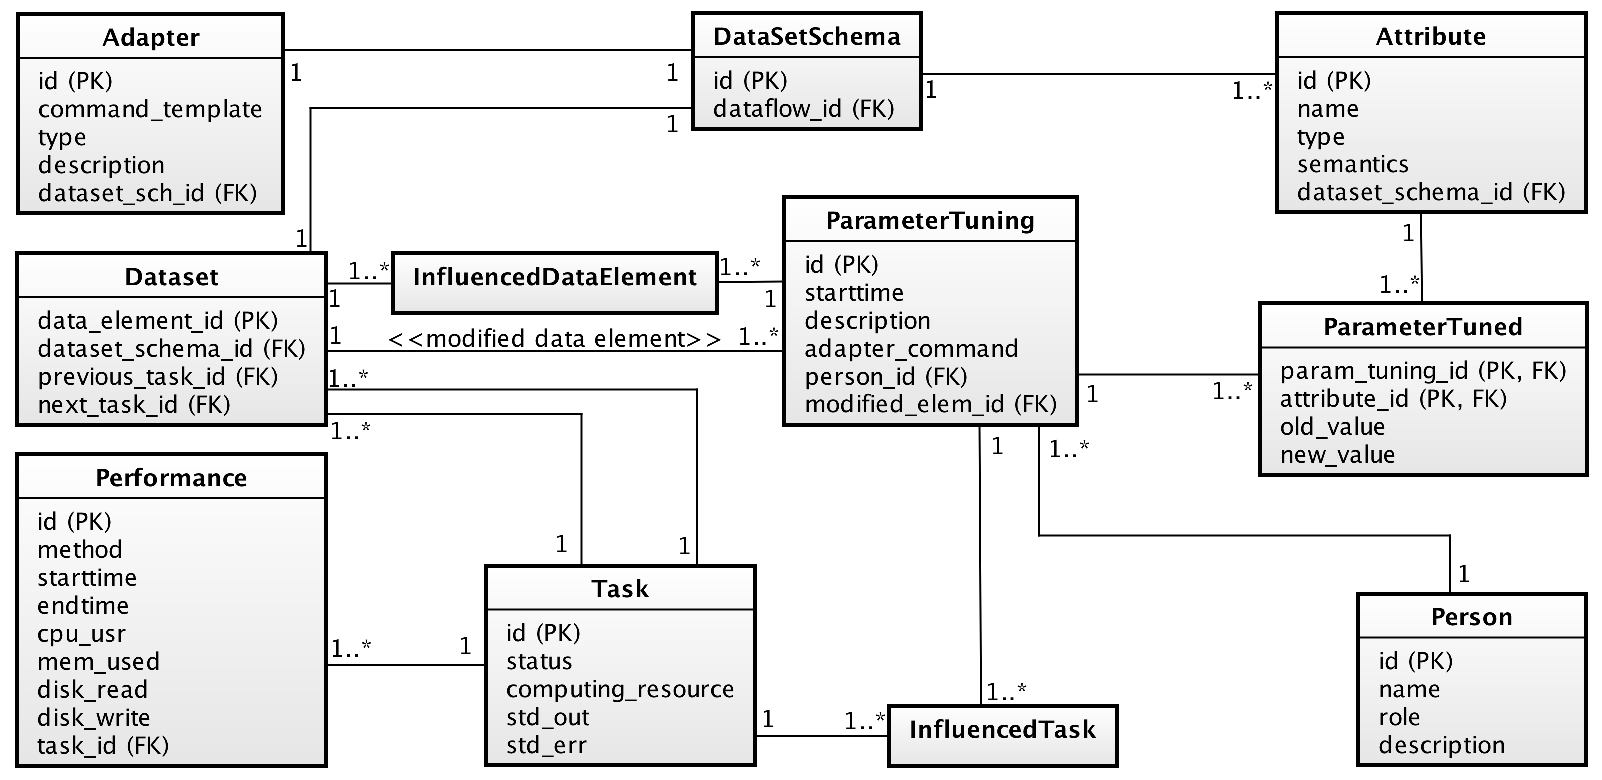
\includegraphics[width=\textwidth,keepaspectratio]{img/DB-Schema-ParameterTuning.png}
    \caption{Workflow Database Schema for DfAdapter.}
    \label{fig:dfadapter_wfdbschema}
\end{figure}

\subsubsection{Combining DfAdapter with DfAnalyzer}


DfAdapter needs a Workflow Data Manager to provide the
data that will give the context of the steering actions, by relating the actions with the overall workflow data being generated during execution.
DfAnalyzer \cite{Silva2017Raw,Camata2018In,silva_dfanalyzer:_2018} follows the dataflow-oriented approach (Sec. \ref{subsec_datacentric}), which is the basis for DfAdapter.
Also, DfAnalyzer follows the same design principles presented in Section \ref{wfscript_system-design-principles} to make data capture efficient, with low execution overhead, and with efficient analytical queries.
Therefore, DfAdapter uses DfAnalyzer as its Workflow Data Manager service with its corresponding Workflow Data Capture API.
In DfAnalyzer, the Workflow Data Manager service is called Provenance Data Extractor and it is accessible via calls from its RESTful data capture API inserted into the workflow script in the analysis points.
Together with the Steering Action Data Capture API inserted in the adaptation points, DfAdapter and DfAnalyzer capture steering action data and data elements in the dataflow from the running workflow, respectively.
Both use the same workflow database, although we modify its schema to add the steering action data-related tables, following the PROV-DfA as in Figure \ref{fig:dfadapter_wfdbschema}.
Finally, during workflow execution, DfAdapter relates and stores the steering action data captured by its Steering Action Data Capture API to the workflow data captured by DfAnalyzer's Workflow Data Capture API in the same integrated workflow database, ready for provenance analyses of the steering actions.


\section{Utilization}
\label{dfadapter_utilization}

To describe how DfAdapter is used, we resort to the methodology in
Section \ref{dfadapter_utilization_methodology}.
We explain how it can be added to dynamic workflows before
execution and how it can be used to manage steering action data.

\textbf{Before execution.} The user identifies a workflow by specifying
parts of the workflow that can be modeled as data transformations and their
datasets, and the data derivation paths. Analysis and adaptation points are added into the workflow script, with their corresponding calls to capture
workflow data and steering action data.
Listing \ref{listing:libmeshcode} shows an example using an excerpt of
libMesh-sedimentation workflow script (Sec. \ref{sub_libmesh}) with the added
data capture calls.
In this example, a programming library to capture the data is imported into the workflow script.
To capture workflow data, it calls DfAnalyzer's Workflow Data Capture API and to capture
steering action data it implements
the Algorithm \ref{alg:alg_tune_operator}, which calls the Steering Action Data Capture API.
The underlying implementation details, \eg{} usage of a programming library,
will depend on the workflow script being instrumented with our API calls. This step is usually
done in collaboration between the workflow specialists and the CSE users, who know how
the code of their workflow script and know which data should be captured and how the calls
should be placed in their script.

\noindent\begin{minipage}[t]{1.0\linewidth}
\begin{lstlisting}[
    language=C++,
    caption={Excerpt of libMesh-sedimentation code with Data Capture API calls.},
    label={listing:libmeshcode}
]
...
for (unsigned int t_step = p.init_tstep;
    (t_step < p.n_time_steps) && (time < p.tmax); t_step++) {
    data_capture_lib.init_time_loop();
    if (parameters_modified()) {
        p = reload_parameters();
        data_capture_lib.capture_steering_time_loop();
    }
    ...
    for (unsigned int nonlinear_step = 0;
        nonlinear_step < p.max_nonlinear_steps; ++nonlinear_step) {
            data_capture_lib.init_fluid_solver();
            flow_system.solve();
            ...
            data_capture_lib.finalize_fluid_solver();
    }
    ...
    data_capture_lib.finalizeTimeLoop();
}
\end{lstlisting}
\end{minipage}


\textbf{During execution\emph{. }}
When the workflow is running, the user
can send an adaptation command using DfAdapter's user interface, which implements the calls to the Adapter API.
DfAdapter's command line-based interface, \codefont{WfSteerCtl},
to be used in a terminal connected to
the HPC machine where the workflow runs.
In the command line, users only
need to inform the input dataset $I_{DS}$ to be adapted, and a
simple key-value data structure containing the parameters and their new
values. For flexibility, the key-value data structure can be passed
directly using the argument \codefont{-\/-p} or can be written into a file to be
passed as an argument. We provide an optional argument \codefont{-\/-reason} to allow
users to annotate that specific steering action.
Listing \ref{listing:dfadapter_commandlines} shows an example
of DfAdapter's command line interface.

\noindent\begin{minipage}[t]{1.0\linewidth}
\begin{lstlisting}[
    language=sh,
    caption={Command lines to use DfAdapter.},
    label={listing:dfadapter_commandlines}
]
$> WfSteerCtl --user="Bob"
$> WfSteerCtl --tune
      --dataset="I_Iteration_Params"
      --p='{"max_linear_iterations": 500}'
      --reason="checking how linear iterations affects
               convergence"
$> echo '{
    "flow_initial_linear_solver_tolerance": 1.0e-6,
    "amr/c_fraction": 1.0e-5
   }' > new-values.json
$> WfSteerCtl --tune
       --dataset="I_Solver"
       --p="new-values.json"

\end{lstlisting}
\end{minipage}




\section{Methodology to Analyze the Overhead}
\label{overhead-analysis-section}

The adoption of our approach depends on how much execution time overhead it
implies. The overhead depends on the data needed for analysis and
adaptation. For analysis, it depends on the workflow data identified in
the workflow script that needs to be captured. That is, which input and
output data values, for each data transformation, should be monitored
during execution. For adaptation, which adaptation points should be added
and how many adaptation actions happened during execution. In
both cases, the overhead depends on data collected for analysis
and adaptation actions, always based on user decisions.

We use the dataflow-oriented concepts (Secs. \ref{subsec_datacentric} and \ref{user_steering_def}) to express the
overhead. Let $\gamma$ be a data transformation execution, \ie{} a task. When a task $\gamma$ is executed to perform a data
transformation $DT_y$, the execution cost of $\gamma$,
$c(\gamma)$, is given by its actual computational cost
$comp(\gamma)$ (\ie{} the inherent cost of
executing $DT_y$) plus the overhead
$o(\gamma)$ introduced because of the utilization of our approach:
\begin{equation}
\label{eq_1}
    c(\gamma) = comp(\gamma) + o(\gamma)
\end{equation}
Let the overhead $o(\gamma)$ of a
task $\gamma$ be expressed as a function of analysis
$anl(\gamma)$ and adaptation adp $s(\gamma)$ overhead introduced in the analysis and adaptation points in the workflow script code, respectively:
\begin{equation}
    o(\gamma) = anl(\gamma) + adp(\gamma)
\end{equation}
The overall overhead is given by the sum of
$o(\gamma)$ for all tasks $\gamma$, of all data
transformations $DT_{y} \in T$. Next, we detail the
analysis and adaptation components.

\textbf{Analysis overhead.}
Analysis overhead
$anl(\gamma)$ is defined by the data capture
overhead $anl_{point}(\gamma)$ and raw data extractions
$ext(\gamma)$ during each data transformation
execution identified by the user as relevant for analysis:
\begin{equation}
    anl(\gamma) = anl_{point}(\gamma) + ext(\gamma)
\end{equation}
Provenance data capture overhead $anl_{point}(\gamma)$ depend
on the number of data values of each data element captured at a task
execution $\gamma$. Each execution $\gamma$ of a data transformation
$DT_y$ consumes input data elements in $I_{DS}$ and produces output
data elements in $I_{DS}$. In DfAdapter, data elements are stored at
once in the beginning (input data elements) and at the end (output data
elements) of each task $\gamma$.

Raw data extraction overhead $ext(\gamma)$ 
depends on the number of data values the user wants to extract from raw
data files at each execution of a data transformation $DT_y$.
Let $V_\gamma$ be the
set of all data values extracted when $\gamma$ is executed. Each
extracted data value $v_i \in V_\gamma$ has an associated data
attribute $a_i$ has semantics in $V_I$ or $V_O$, depending on if
$v_i$ is in a data element in $I_{DS}$ or $O_{DS}$, respectively.
Therefore, the extraction overhead $ext(\gamma)$, for each
$\gamma$ to execute a data transformation $DT_y$ is therefore given by the summation of
costs to extract each $v_i \in V_\gamma$:
\begin{equation}
    ext(\gamma) = \sum_{v_i \in V_\gamma} ext(v_i)
\end{equation}
The cost to extract a data value depends on application-specific raw
data extractors \cite{Silva2017Raw}.


\textbf{Adaptation overhead.} 
The adaptation overhead occurs in
data transformations that have an adaptation point. Adaptation overhead also
depends on when an adaptation action happens.
When an adaptation action
happens, all those operations presented in the sequence diagram in
Figure \ref{fig:dfadapter_seq_diagram} are triggered. 
Let $T' \subset T $ be the subset of the data
transformations that have adaptation points. Then,
\begin{equation}
\label{eq_5}
    adp(\gamma) = adp_{point}(\gamma) + action(\gamma) 
\end{equation}
\noindent 
where 
$adp_{point}(\gamma)$
is the overhead associated
to adding adaptation points to $DT_y$,
$action(\gamma)$
is the overhead associated to
computing that an adaptation action happened, and
$adp_{point}(\gamma) = action(\gamma) = 0, \forall DT_y \notin T'$.



\textbf{Putting it all together.} The overall cost
$c(Df)$ to compute a dataflow $Df$ is
given by the sum of costs to compute the
actual computation $comp(Df)$,
provenance capture $anl_{point}(Df)$, 
raw data extractions $ext(Df)$,
adaptation points $adp_{point}(Df)$,
adaptation actions $action(Df)$
for the entire dataflow $Df$. That is:
\begin{equation} 
\label{final_eq}
\begin{split}
c(Df)   & = comp(Df) + o(Df)                                  \\
        & = comp(Df) + anl(Df) + adp(Df)                     \\
        & = comp(Df) + anl_{point}(Df) + ext(Df) + adp_{point}(Df) + action(Df) 
\end{split}
\end{equation}
\noindent where
$c(Df) = \sum_\gamma c(\gamma)$, for all tasks $\gamma$, for all $DT_y \in T$.
Analogously, the components of
$c(Df)$ can be obtained by the summation of each
individual component for all tasks.
That is,
$anl_{point}(Df) = \sum_\gamma anl_{point}(\gamma)$, 
$ext(Df) = \sum_\gamma ext(\gamma)$,
and so on.

In CSE applications, tasks are often a complex, meaning that for a task $\gamma$, $comp(\gamma)$ takes at least a few
seconds, but often minutes long~\cite{Raicu2008Many-task}.
Experimentally analyzing the individual elapsed time of the components,
$anl_{point}(\gamma), adp_{point}(\gamma), adp_{action}(\gamma)$
of the overhead $o(\gamma)$,
we observe that, on average, they are close to
constant and typically milliseconds-long.
Therefore, we can assume that
in typical CSE applications $comp(\gamma) >> o(\gamma)$, which leads to the generalization that overhead of capturing user steering action data is negligible.
Also,
because such operations occur asynchronously and in a different
computing resource, the time for the individual components of
$o(\gamma)$ is ``hidden'' by the actual computation, which
is significantly higher. This contributes to reduce the impact on the
workflow execution performance.
If we consider $ext(Df)$  which depends on
the user settings, it is still typically very much smaller than the raw
data that is being generated and stored on files. As we show in our real
case study (Sec. \ref{sec_overhead_eval_wokflow_script}), the overall $o(Df)$, including the
costs for $ext(Df)$, is less than 2\%, which is still negligible.





In the next chapter, we present the second instantiation of WfSteer to support a data-centric WMS.